\documentclass[11pt,a4paper]{article}

\usepackage[danish]{babel}
\usepackage[T1]{fontenc}
\usepackage[utf8]{inputenc}
\usepackage{icomma}
\usepackage{amsmath, amssymb, mathtools}
\usepackage{booktabs, enumitem}
\usepackage{graphicx}
\usepackage{xcolor}
\usepackage[most]{tcolorbox}
\tcbuselibrary{skins, breakable}
\usepackage{tikz}
\usetikzlibrary{calc, arrows.meta, positioning}
\usepackage{pgfplots}
\pgfplotsset{compat=1.18}
\usepackage[hidelinks]{hyperref}
\usepackage[capitalise]{cleveref}
\usepackage{geometry}
\geometry{a4paper, margin=2.3cm}
\usepackage{parskip}
\usepackage{multicol}
\usepackage{titlesec}
\usepackage{fancyhdr}

% ── farver (hus-palette fra gxu-funktioner-og-ligninger.tex) ────────────────
\definecolor{gxu-paper}{HTML}{F7F9FB}
\definecolor{gxu-ink}{HTML}{1A1F2B}
\definecolor{gxu-inksoft}{HTML}{4A5568}
\definecolor{gxu-accent}{HTML}{58C4DD}
\definecolor{gxu-purple}{HTML}{7C5CFC}
\definecolor{gxu-red}{HTML}{C0392B}
\definecolor{boxframe}{HTML}{CBD5E0}

% alias
\definecolor{accent}{HTML}{58C4DD}
\definecolor{accentdark}{HTML}{2A8FB8}
\definecolor{ink}{HTML}{1A1F2B}
\definecolor{inksoft}{HTML}{4A5568}
\definecolor{boxbg}{HTML}{F7F9FB}

% ── boks-stil ───────────────────────────────────────────────────────────────
\newtcolorbox{opgavebox}{
  enhanced, breakable,
  colback=boxbg, colframe=boxframe,
  boxrule=0.4pt, arc=2pt, left=4pt, right=4pt, top=3pt, bottom=3pt,
  before skip=8pt, after skip=8pt
}
\newtcolorbox{regelbox}{
  enhanced, breakable,
  colback=boxbg, colframe=accent,
  boxrule=0.6pt, arc=2pt, left=6pt, right=6pt, top=4pt, bottom=4pt,
  before skip=8pt, after skip=8pt
}

% ── titel-stil ──────────────────────────────────────────────────────────────
\titleformat{\section}{\Large\bfseries\color{gxu-accent}}{\thesection}{0.6em}{}
\titleformat{\subsection}{\large\bfseries\color{gxu-accent}}{\thesubsection}{0.6em}{}
\titlespacing*{\section}{0pt}{1.1em}{0.5em}
\titlespacing*{\subsection}{0pt}{0.8em}{0.4em}

% ── header / footer ─────────────────────────────────────────────────────────
\pagestyle{fancy}
\fancyhf{}
\fancyhead[L]{\sffamily\small\color{gxu-inksoft}GXU -- Matematik}
\fancyhead[R]{\sffamily\small\color{gxu-inksoft}Træningsopgavesæt 6}
\fancyfoot[C]{\sffamily\small\color{gxu-inksoft}\thepage}
\renewcommand{\headrulewidth}{0.0pt}

% ── makroer ─────────────────────────────────────────────────────────────────
\makeatletter
\newcommand{\eq}[2]{\begin{equation}#2\tag{#1}\end{equation}}
\makeatother

% Kompetence-chip
\newcommand{\kompetence}[1]{%
  \tcbox[on line, colback=gxu-accent!15, colframe=gxu-accent, boxrule=0.4pt,
         arc=10pt, left=6pt, right=6pt, top=3pt, bottom=3pt, boxsep=0pt,
         fontupper=\sffamily\small]{#1}\hspace{5pt}%
}

% CAS-chip: markerer at opgaven maa loeses med hjælpemidler
\newcommand{\cas}{%
  \tikz[baseline=-0.6ex]\node[draw=gxu-purple, fill=gxu-purple!12,
    rounded corners=3pt, inner xsep=4pt, inner ysep=1.2pt,
    font=\sffamily\scriptsize, text=gxu-purple] {CAS};%
}
\newcommand{\casnote}[1]{{\small\color{gxu-purple}\itshape #1}}

\title{}
\author{}
\date{}

\begin{document}

\begin{center}
  {(\Large\bfseries Træningsopgavesæt 6)}\\[2pt]
  {\color{inksoft}\large Differentialregning}\\[6pt]
  {\color{inksoft}\small 1.--2.\ g \quad -- \quad Mat B \quad -- \quad
   Fra Omar og Karoline --- 18.~november 2026}
\end{center}

\vspace{6pt}
\hrule height 0.4pt
\vspace{10pt}

\noindent
Dette sæt gennemgår differentialregning fra bunden: hvad en afledning
overhovedet er, hvordan man regner den, og hvad man bruger den til. Hvert
emne starter med en kort regel og et udregnet eksempel --- så kan du løse
opgaverne på samme måde. Alle facit ligger bagerst.

\vspace{6pt}
\noindent
{\small\color{inksoft}\textit{Sådan bruger du sættet: Læs reglen, kig på
eksemplet, og brug derefter samme metode på opgaverne. Skriv alle
mellemregninger ned. Opgaver med en lilla \cas{}-mærke må du løse med
hjælpemidler (GeoGebra eller TI-Nspire) --- resten skal du regne i hånden.}}
\par\vspace{4pt}
\noindent
\casnote{Markeringen står for "hjælpemidler tilladt", som i den skriftlige
prøve på mat B: der er dels en del uden hjælpemidler og dels en del med.}

% ═════════════════════════════════════════════════════════════════════════════
\section{Hvad er en afledning?}
% ═════════════════════════════════════════════════════════════════════════════

\kompetence{Problembehandling} \kompetence{Ræsonnement}

\noindent
En afledning $f'(x)$ er \emph{hældningen} i et punkt. Hældningen kan vi
finde som en grænseværdi af sekantens hældning, når den anden ende af
sekanten flytter ind mod punktet.

\begin{regelbox}
\textbf{Definition:} For $f(x) = x^{2}$ er sekanten gennem $(0,0)$ og
$(2,4)$ en linje med hældningen $\frac{4-0}{2-0} = 2$. Når den anden ende
flytter ind mod $(0,0)$, bliver hældningen $2$. Vi siger, at $f'(0) = 2$.

\textbf{Formel:} \quad
$f'(x) = \displaystyle\lim_{h \to 0} \frac{f(x+h) - f(x)}{h}$
\end{regelbox}

\textbf{Eksempel: Beregn $f'(x)$ for $f(x) = x^{2}$ ved definitionen.}

\begin{align*}
  f'(x) &= \lim_{h \to 0} \frac{(x+h)^{2} - x^{2}}{h}\\[4pt]
        &= \lim_{h \to 0} \frac{x^{2} + 2xh + h^{2} - x^{2}}{h}\\[4pt]
        &= \lim_{h \to 0} \frac{2xh + h^{2}}{h}\\[4pt]
        &= \lim_{h \to 0} (2x + h) = 2x
\end{align*}

Tjek: $f'(x) = 2x$ er netop hældningen i $(x, x^{2})$. Grafen er en
parabel, og hældningen vokser lineært med $x$ --- det passer.

\vspace{4pt}
\noindent
\textbf{Sekant og tangent:} På figuren er $P = (1,1)$ et fast punkt på
parablen, og $Q = (3,9)$ et andet punkt. Sekanten gennem $P$ og $Q$ har
hældningen $\frac{9-1}{3-1} = 4$, mens tangenten i $P$ har hældningen
$f'(1) = 2$. Jo tættere $Q$ flytter hen mod $P$, desto tættere kommer
sekanten på tangenten.

\begin{center}
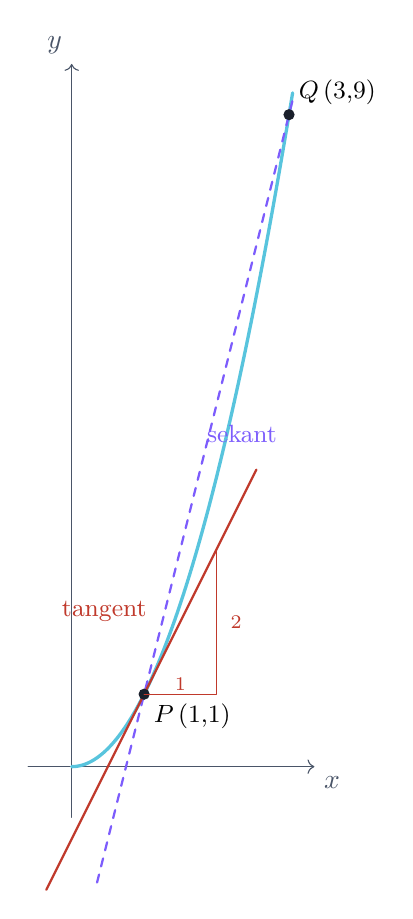
\begin{tikzpicture}[scale=0.92, line cap=round, line join=round]
  % akser
  \draw[->, thin, inksoft] (-0.6,0) -- (3.35,0) node[below right] {$x$};
  \draw[->, thin, inksoft] (0,-0.7) -- (0,9.7) node[above left] {$y$};
  % parabel f(x)=x^2
  \draw[accent, very thick, domain=0:3.05, samples=80, variable=\x]
    plot ({\x},{\x*\x});
  % sekant gennem P(1,1) og Q(3,9): y = 4x-3
  \draw[gxu-purple, thick, dashed, domain=0.35:3.05, samples=40, variable=\x]
    plot ({\x},{4*\x-3});
  % tangent i P(1,1): y = 2x-1
  \draw[gxu-red, thick, domain=-0.35:2.55, samples=40, variable=\x]
    plot ({\x},{2*\x-1});
  % punkter
  \fill[gxu-ink] (1,1) circle (2.2pt);
  \fill[gxu-ink] (3,9) circle (2.2pt);
  \node[below right, font=\small] at (1,1) {$P\,(1,1)$};
  \node[above right, font=\small] at (3,9) {$Q\,(3,9)$};
  % etiketter
  \node[gxu-red, font=\small] at (0.45,2.15) {tangent};
  \node[gxu-purple, font=\small] at (2.35,4.6) {sekant};
  % haeldningstrekant paa tangenten
  \draw[thin, gxu-red] (1,1) -- (2,1) -- (2,3);
  \node[right, font=\scriptsize, text=gxu-red] at (2.06,2) {$2$};
  \node[above, font=\scriptsize, text=gxu-red, inner sep=1pt] at (1.5,1) {$1$};
\end{tikzpicture}
\end{center}

\begin{opgavebox}
\textbf{Opgave 1.1} \quad Beregn $f'(x)$ for $f(x) = x^{2} + 3x$ ved
definitionen. \hfill {\small\color{inksoft}(Start med at skrive
$f(x+h)$ ud.)}
\end{opgavebox}

\begin{opgavebox}
\textbf{Opgave 1.2} \quad Beregn $f'(x)$ for $f(x) = 3x - 5$ ved
definitionen.
\end{opgavebox}

\begin{opgavebox}
\textbf{Opgave 1.3} \quad Beregn $f'(x)$ for $f(x) = x^{3}$ ved definitionen.
\end{opgavebox}

\begin{opgavebox}
\textbf{Opgave 1.4} \quad For $f(x) = x^{3}$ er sekanten gennem $(1,1)$ og
$(2,8)$. \quad (a) Beregn sekantens hældning. \quad (b) Beregn $f'(1)$ og
$f'(2)$. \quad (c) Hvorimellem ligger sekantens hældning --- og hvorfor er
det et rimeligt svar?
\end{opgavebox}

\begin{opgavebox}
\textbf{Opgave 1.5} \quad \cas \quad Beregn $f'(2)$ for $f(x) = x^{3}$
numerisk, altså med grænseværdien. Sæt $h = 0{,}1$, $h = 0{,}01$ og
$h = 0{,}001$, og sammenlign med din svar fra Opgave 1.3.
\end{opgavebox}

\begin{opgavebox}
\textbf{Opgave 1.6} \quad For $f(x) = x^{2} - 4x + 7$ er $f'(x) = 2x - 4$.
Find de $x$-værdier, hvor hældningen er $3$, hvor den er $0$, og hvor den
er $-3$. \hfill {\small\color{inksoft}(Lav en lille tabel med $x$ og
$f'(x)$.)}
\end{opgavebox}

% ═════════════════════════════════════════════════════════════════════════════
\section{Afledningsregler}
% ═════════════════════════════════════════════════════════════════════════════

\kompetence{Regning} \kompetence{Hjælpemidler}

\noindent
Når vi kender reglerne, slipper vi for at gå til definitionen hver gang.

\begin{regelbox}
\textbf{Sum:} \quad $(f + g)' = f' + g'$ \\[3pt]
\textbf{Konstant:} \quad $(c \cdot f)' = c \cdot f'$ \\[3pt]
\textbf{Potens:} \quad $(x^{n})' = n \cdot x^{n-1}$ \\[3pt]
\textbf{Eksponential:} \quad $(e^{x})' = e^{x}$, \quad $(a^{x})' = a^{x} \ln a$
\\[3pt]
\textbf{Logaritme:} \quad $(\ln x)' = \frac{1}{x}$
\end{regelbox}

\textbf{Eksempel: Summer og potens}
\begin{align*}
  f(x) &= 4x^{3} - 2x + 7\\
  f'(x) &= 3 \cdot 4x^{2} - 2 = 12x^{2} - 2
\end{align*}

\subsection*{Produktregelen}

\begin{regelbox}
\textbf{Regel:} Når begge faktorer afhænger af $x$, ganger du hver del med
den anden faktorens afledning og lægger sammen:
$(f \cdot g)' = f' \cdot g + f \cdot g'$.
\end{regelbox}

\textbf{Eksempel: $f(x) = x^{2}(2x + 1)$}
\begin{align*}
  f(x) &= x^{2}(2x+1) = 2x^{3} + x^{2}\\
  f'(x) &= 3 \cdot 2x^{2} + 2x = 6x^{2} + 2x
\end{align*}
Tjek med produktregelen: $2x \cdot (2x+1) + x^{2} \cdot 2 = 4x^{2} + 2x +
2x^{2} = 6x^{2} + 2x$ \checkmark

\subsection*{Kvotientreglen}

\begin{regelbox}
\textbf{Regel:} $\left(\frac{f}{g}\right)' = \dfrac{f' \cdot g - f \cdot g'}{g^{2}}$.
Hold nævneren i anden potens, og pas på fortegnet --- den er
$\text{numerator} \cdot g - \text{numerator} \cdot g'$, ikke plus.
\end{regelbox}

\textbf{Eksempel: $f(x) = \dfrac{x^{2}+1}{x-1}$}
\begin{align*}
  f'(x) &= \frac{2x \cdot (x-1) - (x^{2}+1) \cdot 1}{(x-1)^{2}}\\[4pt]
        &= \frac{2x^{2} - 2x - x^{2} - 1}{(x-1)^{2}}
         = \frac{x^{2} - 2x - 1}{(x-1)^{2}}
\end{align*}

\begin{opgavebox}
\textbf{Opgave 2.1} \quad Bestem $f'(x)$ for $f(x) = 5x^{3} - 3x$.
\end{opgavebox}

\begin{opgavebox}
\textbf{Opgave 2.2} \quad Bestem $f'(x)$ for $f(x) = x^{4} - 2x^{2} + 7$.
\end{opgavebox}

\begin{opgavebox}
\textbf{Opgave 2.3} \quad Bestem $f'(x)$ for $f(x) = x^{2}(2x+1)$ --- brug
produktregelen.
\end{opgavebox}

\begin{opgavebox}
\textbf{Opgave 2.4} \quad \cas \quad Bestem $f'(x)$ for $f(x) = x^{3}e^{x}$.
\end{opgavebox}

\begin{opgavebox}
\textbf{Opgave 2.5} \quad Bestem $f'(x)$ for $f(x) = \dfrac{x^{2}+1}{x-1}$
--- brug kvotientreglen.
\end{opgavebox}

\begin{opgavebox}
\textbf{Opgave 2.6} \quad Bestem $f'(x)$ for $f(x) = 2e^{3x}$ og for
$g(x) = \ln(3x)$.
\end{opgavebox}

\begin{opgavebox}
\textbf{Opgave 2.7} \quad Bestem $f'(x)$ for $f(x) = e^{x} + 3\ln(x)$.
\end{opgavebox}

% ═════════════════════════════════════════════════════════════════════════════
\section{Kæderegelen}
% ═════════════════════════════════════════════════════════════════════════════

\kompetence{Regning} \kompetence{Ræsonnement}

\noindent
Når en funktion er bygget op inde i en anden, taler vi om en
\emph{sammensætning}: $f(g(x))$. Kæderegelen lader os aflede lag for lag.

\begin{regelbox}
\textbf{Regel:} $\left(f \circ g\right)'(x) = f'\!\left(g(x)\right) \cdot g'(x)$.
\textbf{Læs inde indefladsen indefølge:} afled den ydre funktion, sæt den
indre funktion ind i stedet for variablen, og gang med den indre funktions
afledning.
\end{regelbox}

\textbf{Eksempel: $f(x) = (x^{2}+1)^{3}$}
\begin{align*}
  f'(x) &= 3(x^{2}+1)^{2} \cdot 2x &&\text{(ydre: potensreglen)}\\
        &= 6x(x^{2}+1)^{2}   &&\text{(indre: afled af $x^{2}+1$)}
\end{align*}

\subsection*{Et par almindelige sammensætninger}

\begin{center}
\renewcommand{\arraystretch}{1.35}
\begin{tabular}{@{}lll@{}}
\toprule
\textbf{Funktion} & \textbf{Afledning} & \textbf{Ræsonnement} \\
\midrule
$(x^{2}+1)^{3}$  & $6x(x^{2}+1)^{2}$ & potensreglen ind i potensreglen \\
$e^{x^{2}}$      & $2x \cdot e^{x^{2}}$ & eksponential ind i eksponential \\
$\ln(2x+1)$      & $\dfrac{2}{2x+1}$ & logaritme ind i lineær \\
$\sqrt{x^{2}+1}$  & $\dfrac{x}{\sqrt{x^{2}+1}}$ & potens $\frac{1}{2}$ ind i andengrad \\
\bottomrule
\end{tabular}
\end{center}

\begin{opgavebox}
\textbf{Opgave 3.1} \quad Bestem $f'(x)$ for $f(x) = (2x+3)^{5}$.
\end{opgavebox}

\begin{opgavebox}
\textbf{Opgave 3.2} \quad Bestem $f'(x)$ for $f(x) = e^{x^{2}+1}$.
\end{opgavebox}

\begin{opgavebox}
\textbf{Opgave 3.3} \quad Bestem $f'(x)$ for $f(x) = \ln(2x^{2}+1)$.
\end{opgavebox}

\begin{opgavebox}
\textbf{Opgave 3.4} \quad Bestem $f'(x)$ for $f(x) = \sqrt{x^{2}+1}$.
\end{opgavebox}

\begin{opgavebox}
\textbf{Opgave 3.5} \quad Bestem $f'(x)$ for $f(x) = \ln(x^{2})$. \hfill
{\small\color{inksoft}(Husk at undersøge, hvor $f$ er defineret --- og om
afledningen findes overalt.)}
\end{opgavebox}

\begin{opgavebox}
\textbf{Opgave 3.6} \quad \cas \quad Bestem $f'(x)$ for
$f(x) = \dfrac{(x^{2}+4)^{3}}{x-1}$. \hfill
{\small\color{inksoft}(Skriv kvotientreglen op først --- og overvej om
kæderegelen også kan bruges inde i.)}
\end{opgavebox}

\begin{opgavebox}
\textbf{Opgave 3.7} \quad Bestem $f'(x)$ for $f(x) = x^{2}\ln(x)$.
\end{opgavebox}

% ═════════════════════════════════════════════════════════════════════════════
\section{Tangent og normal}
% ═════════════════════════════════════════════════════════════════════════════

\kompetence{Problembehandling} \kompetence{Modellering}

\noindent
En tangentlinje i et punkt $(x_{0}, f(x_{0}))$ er den linje, der netop
rører grafen i punktet. Normalen står vinkelret på tangenten.

\begin{regelbox}
\textbf{Tangentlinjen:} \quad
$y = f'(x_{0}) \cdot (x - x_{0}) + f(x_{0})$ \\[4pt]
\textbf{Normalen:} \quad hældningen er $\dfrac{-1}{f'(x_{0})}$, og den
går gennem det samme punkt.
\end{regelbox}

\textbf{Eksempel: $f(x) = x^{2}+3x$, tangent og normal i $x_{0} = 1$}
\begin{align*}
  f(1) &= 1 + 3 = 4, & f'(x) &= 2x + 3, & f'(1) &= 5\\[4pt]
  \text{Tangent:} \quad y &= 5(x-1) + 4 = 5x - 1\\[4pt]
  \text{Normal:} \quad y &= -\tfrac{1}{5}(x-1) + 4
\end{align*}

\begin{center}
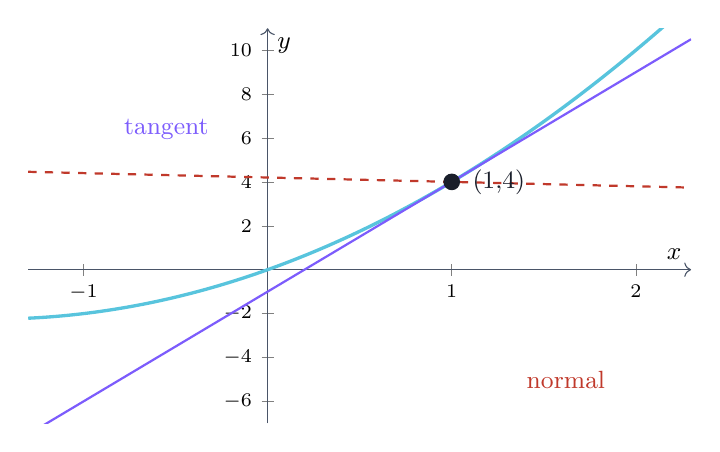
\begin{tikzpicture}
\begin{axis}[
  width=10cm, height=6.6cm,
  axis lines=middle,
  xmin=-1.3, xmax=2.3, ymin=-7, ymax=11,
  xtick={-1,0,1,2}, ytick={-6,-4,-2,0,2,4,6,8,10},
  xlabel={$x$}, ylabel={$y$},
  tick label style={font=\scriptsize},
  label style={font=\small},
  axis line style={->, thin, inksoft},
  every axis plot/.append style={line width=1.2pt},
  clip=true
]
  \addplot[accent, very thick, domain=-1.3:2.3, samples=120] {x^2+3*x};
  \addplot[gxu-purple, thick, domain=-1.3:2.3, samples=2] {5*x-1};
  \addplot[gxu-red, thick, dashed, domain=-1.3:2.3, samples=2] {-0.2*x+4.2};
  \addplot[only marks, mark=*, mark size=2.4pt, gxu-ink] coordinates {(1,4)};
  \node[font=\small, text=gxu-purple] at (axis cs:-0.55,6.4) {tangent};
  \node[font=\small, text=gxu-red] at (axis cs:1.62,-5.0) {normal};
  \node[font=\small, text=ink, anchor=west] at (axis cs:1.06,4.0) {$(1,4)$};
\end{axis}
\end{tikzpicture}
\end{center}

\begin{opgavebox}
\textbf{Opgave 4.1} \quad Bestem tangentlinjen og normalen i $x_{0} = 1$
for $f(x) = x^{2} + 3x$.
\end{opgavebox}

\begin{opgavebox}
\textbf{Opgave 4.2} \quad Bestem tangentlinjen og normalen i $x_{0} = 2$
for $f(x) = x^{3} - 3x$.
\end{opgavebox}

\begin{opgavebox}
\textbf{Opgave 4.3} \quad Bestem tangentlinjen i $x_{0} = 0$ for
$f(x) = e^{x}$, og bestem også normalens hældning.
\end{opgavebox}

\begin{opgavebox}
\textbf{Opgave 4.4} \quad For hvilket $x_{0}$ er tangentlinjen til
$f(x) = x^{2} - 4x + 7$ vandret? \hfill
{\small\color{inksoft}(Vandret betyder hældningen $0$.)}
\end{opgavebox}

\begin{opgavebox}
\textbf{Opgave 4.5} \quad Bestem tangentlinjen i $x_{0} = 1$ for
$f(x) = \ln(x)$. Hvor skærer den y-aksen, og hvad er normalens hældning?
\end{opgavebox}

\begin{opgavebox}
\textbf{Opgave 4.6} \quad Tangentlinjen i $x_{0} = 1$ for
$f(x) = x^{2} + 3x$ er $y = 5x - 1$. \quad (a) Hvilket punkt på
x-aksen skærer den? \quad (b) Normalen i samme punkt er
$y = -\tfrac{1}{5}(x-1) + 4$. Hvor skærer den y-aksen?
\end{opgavebox}

\begin{opgavebox}
\textbf{Opgave 4.7} \quad For hvilke $x_{0}$ går tangentlinjen til
$f(x) = x^{2} - 4x + 7$ gennem punktet $(0,0)$? \hfill
{\small\color{inksoft}(Sæt $f(x_{0}) - f'(x_{0}) \cdot x_{0} = 0$ --- det er
ligesom at kræve, at tangentlinjen går gennem $(0,0)$.)}
\end{opgavebox}

% ═════════════════════════════════════════════════════════════════════════════
\section{Monotoniforhold}
% �════════════════════════════════════════════════════════════════════════════

\kompetence{Ræsonnement} \kompetence{Repræsentation}

\noindent
En voksende graf har positiv afledning, en faldende har negativ. Vi
finder derfor først de punkter, hvor $f'(x) = 0$, og deler aksen op i
intervaller imellem dem.

\begin{regelbox}
\textbf{Regel:} \quad
$f'(x) > 0$ \quad$\Rightarrow$ \quad $f$ er stigende \qquad og \qquad
$f'(x) < 0$ \quad$\Rightarrow$ \quad $f$ er faldende.
Tegn et \emph{sign skema} for $f'$: sæt et nulpunkt for hver rod af $f'$,
og skriv $+$ og $-$ mellem punkterne.
\end{regelbox}

\textbf{Eksempel: $f(x) = x^{3} - 3x + 1$}
\begin{align*}
  f'(x) &= 3x^{2} - 3 = 3(x-1)(x+1)
\end{align*}
Nulpunkter er $x = -1$ og $x = 1$. Vi tester ét tal i hvert interval:

\begin{center}
\begin{tikzpicture}[>=Stealth, line cap=round]
  \draw[very thick, inksoft] (-4.3,0) -- (4.3,0);
  \node[below right, font=\small] at (4.2,0) {$x$};
  \foreach \x/\lab in {-1/{$-1$},1/{$1$}} {
    \draw[very thick, inksoft] (\x,-0.22) -- (\x,0.22);
    \node[below, font=\small] at (\x,-0.28) {\lab};
  }
  \node[above, font=\small, text=accentdark] at (-2.7,0.28) {$+$};
  \node[above, font=\small, text=gxu-red]   at ( 0,0.28) {$-$};
  \node[above, font=\small, text=accentdark] at ( 2.7,0.28) {$+$};
  \node[above, font=\small, text=inksoft] at (0,0.95) {$f'(x)$};
\end{tikzpicture}
\end{center}

\begin{align*}
  x < -1 &: \quad f'(-2) = 9 > 0 \quad\Rightarrow \text{stigende}\\
  -1 < x < 1 &: \quad f'(0) = -3 < 0 \quad\Rightarrow \text{faldende}\\
  x > 1 &: \quad f'(2) = 9 > 0 \quad\Rightarrow \text{stigende}
\end{align*}

\begin{opgavebox}
\textbf{Opgave 5.1} \quad Bestem monotoniforhold for $f(x) = x^{2} - 4x$.
\end{opgavebox}

\begin{opgavebox}
\textbf{Opgave 5.2} \quad Bestem monotoniforhold for
$f(x) = x^{3} - 6x^{2} + 9x$.
\end{opgavebox}

\begin{opgavebox}
\textbf{Opgave 5.3} \quad Bestem monotoniforhold for $f(x) = x^{3} + 3x$.
\hfill {\small\color{inksoft}(Kan $f'$ have nogen nulpunkter?)}
\end{opgavebox}

\begin{opgavebox}
\textbf{Opgave 5.4} \quad Bestem monotoniforhold for $f(x) = e^{x} - x$, og
finds den mindste værdi af $f$.
\end{opgavebox}

\begin{opgavebox}
\textbf{Opgave 5.5} \quad Bestem monotoniforhold for $f(x) = x^{3} - 3x + 1$.
\end{opgavebox}

\begin{opgavebox}
\textbf{Opgave 5.6} \quad \cas \quad Bestem monotoniforhold for
$f(x) = x^{3} - 3x^{2} - 9x + 5$. \hfill
{\small\color{inksoft}(Tegn et sign skema og forklar dine valg.)}
\end{opgavebox}

% ═════════════════════════════════════════════════════════════════════════════
\section{Ekstrema}
% ═════════════════════════════════════════════════════════════════════════════

\kompetence{Problembehandling} \kompetence{Modellering}

\noindent
Et \emph{stationært punkt} er et punkt, hvor $f'(x_{0}) = 0$. Det kan være
et maximum, et minimum, eller et såkaldt saddelpunkt.

\begin{regelbox}
\textbf{Regel:} Find de stationære punkter ved at sætte $f'(x) = 0$. Test
så hvert punkt med $f''$:
\\[2pt]
$f''(x_{0}) < 0$ \quad$\Rightarrow$ \quad\emph{lokalt maximum}, \qquad
$f''(x_{0}) > 0$ \quad$\Rightarrow$ \quad\emph{lokalt minimum}.
\end{regelbox}

\textbf{Eksempel: $f(x) = x^{3} - 3x + 1$}
\begin{align*}
  f'(x) &= 3x^{2} - 3 = 0 \quad\Rightarrow\quad x = \pm 1\\[4pt]
  f''(x) &= 6x\\[4pt]
  f''(-1) &= -6 < 0 \quad\Rightarrow \quad \text{lokalt max i } (-1,\, 3)\\
  f''(1) &= 6 > 0 \quad\Rightarrow \quad \text{lokalt min i } (1,\, -1)
\end{align*}

\begin{center}
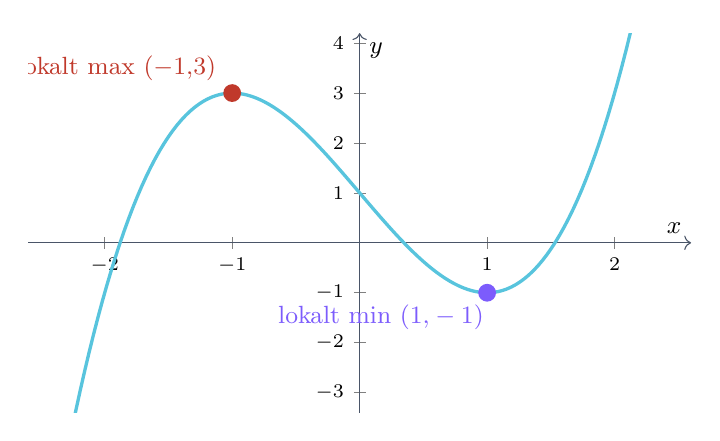
\begin{tikzpicture}
\begin{axis}[
  width=10cm, height=6.4cm,
  axis lines=middle,
  xmin=-2.6, xmax=2.6, ymin=-3.4, ymax=4.2,
  xtick={-2,-1,0,1,2}, ytick={-3,-2,-1,0,1,2,3,4},
  xlabel={$x$}, ylabel={$y$},
  tick label style={font=\scriptsize},
  label style={font=\small},
  axis line style={->, thin, inksoft},
  every axis plot/.append style={line width=1.2pt},
  clip=true
]
  \addplot[accent, very thick, domain=-2.4:2.4, samples=140] {x^3-3*x+1};
  \addplot[only marks, mark=*, mark size=2.6pt, gxu-red]  coordinates {(-1,3)};
  \addplot[only marks, mark=*, mark size=2.6pt, gxu-purple] coordinates {(1,-1)};
  \node[font=\small, text=gxu-red, anchor=south east] at (axis cs:-1.05,3.05)
    {lokalt max $(-1,3)$};
  \node[font=\small, text=gxu-purple, anchor=north east] at (axis cs:1.05,-1.05)
    {lokalt min $(1,-1)$};
\end{axis}
\end{tikzpicture}
\end{center}

\begin{opgavebox}
\textbf{Opgave 6.1} \quad Bestem de stationære punkter for
$f(x) = x^{2} - 4x + 1$, og klassificér dem.
\end{opgavebox}

\begin{opgavebox}
\textbf{Opgave 6.2} \quad Bestem de stationære punkter for
$f(x) = x^{3} - 6x^{2} + 9x$, og klassificér dem.
\end{opgavebox}

\begin{opgavebox}
\textbf{Opgave 6.3} \quad Bestem de stationære punkter for
$f(x) = x^{3} - 3x^{2} + 4x$, og klassificér dem. \hfill
{\small\color{inksoft}(Undersøg diskriminanten i $f'(x) = 0$.)}
\end{opgavebox}

\begin{opgavebox}
\textbf{Opgave 6.4} \quad Bestem de stationære punkter for
$f(x) = x^{2}(x-3)^{2}$, og klassificér dem. \hfill
{\small\color{inksoft}(Skriv $f$ ud som et polynomium først.)}
\end{opgavebox}

\begin{opgavebox}
\textbf{Opgave 6.5} \quad Bestem de stationære punkter for
$f(x) = x \cdot e^{x}$, og klassificér dem.
\end{opgavebox}

\begin{opgavebox}
\textbf{Opgave 6.6} \quad \cas \quad Bestem de stationære punkter for
$f(x) = x^{3} - 3x^{2} - 9x + 5$, og klassificér dem.
\end{opgavebox}

% ═════════════════════════════════════════════════════════════════════════════
\section{Optimering}
% ═════════════════════════════════════════════════════════════════════════════

\kompetence{Modellering} \kompetence{Problembehandling}

\noindent
Optimering er der, hvor differentialregningen bruges til noget: vi vil
finde den bedste løsning, og afledningen fortæller os, hvor vi skal kigge.

\begin{regelbox}
\textbf{Metoden:} \quad
\textbf{(1)} Definér variablen: hvad er $x$, og hvad er fast? \quad
\textbf{(2)} Opskriv den funktion, du vil optimere. \quad
\textbf{(3)} Afled, og find $f'(x) = 0$. \quad
\textbf{(4)} Tjek med $f''$ (eller med et sign skema), at det er det
ekstremum, du leder efter. \quad
\textbf{(5)} Svar med enhed, og tjek at svaret er realistisk.
\end{regelbox}

\textbf{Eksempel: En rektangulær have med omkreds $40$ m.}
Hvis den ene side er $x$, er den anden $20 - x$, og arealet er
$A(x) = x(20 - x) = 20x - x^{2}$.
\begin{align*}
  A'(x) &= 20 - 2x = 0 \quad\Rightarrow\quad x = 10\\[4pt]
  A''(x) &= -2 < 0 \quad\Rightarrow\quad \text{lokalt maximum}\\[4pt]
  A(10) &= 20 \cdot 10 - 10^{2} = 100\,\text{m}^{2}
\end{align*}
Tjek: $10 \cdot 10 = 100 > 0$, så arealet er positivt, og $10 + 10 = 20$,
så omkredsen er $40$ m. Kvadratet er det største rektangel med omkreds $40$
m --- det kan man tjekke ved at sammenligne med et rektangel $14 \times 6$,
der har omkreds $40$ m men kun $84\,\text{m}^{2}$.

\subsection*{Gå altid tilbage til modellen}

En tangentlinje er et \emph{vejledende} svar, ikke en løsning. Når du har
fundet $x$, skal du:

\begin{itemize}[leftmargin=2em, itemsep=1pt]
  \item sætte $x$ tilbage i den oprindelige funktion (ikke i afledningen),
  \item kontrollere at $x$ giver en fornuftig løsning i situationen --- fx at
  en længde ikke bliver negativ,
  \item svare med den rigtige enhed.
\end{itemize}

\begin{opgavebox}
\textbf{Opgave 7.1} \quad En have er rektangulær og har omkreds $24$ m.
Den ene side er $x$. \quad (a) Opskriv arealet som funktion af $x$.
\quad (b) Find det maksimale areal. \hfill
{\small\color{inksoft}(Skriv $24 - 2x$ for den anden side.)}
\end{opgavebox}

\begin{opgavebox}
\textbf{Opgave 7.2} \quad \cas \quad En cylindrisk beholder \emph{uden låg}
skal rumme $1\,000\,\text{cm}^{3}$. Find den beholder, der bruger mindst
materiale, altså har mindst overflade. \hfill
{\small\color{inksoft}(Radius $r$, højde $h$, overflade
$\pi r^{2} + 2\pi r h$.)}
\end{opgavebox}

\begin{opgavebox}
\textbf{Opgave 7.3} \quad En kasse med kvadratisk bund skal rumme
$64\,\text{cm}^{3}$. Find den kasse, der har mindst overflade. \hfill
{\small\color{inksoft}(Bundens side er $x$, så højden er $h = 64/x^{2}$.)}
\end{opgavebox}

\begin{opgavebox}
\textbf{Opgave 7.4} \quad \cas \quad En retvinklet trekant har hypotenusen
$10$ cm. Find den, der har størst areal. \hfill
{\small\color{inksoft}(Sæt $a$ til den ene ben og $b$ til det andet, så
$a^{2} + b^{2} = 100$.)}
\end{opgavebox}

\begin{opgavebox}
\textbf{Opgave 7.5} \quad En have på $200\,\text{m}^{2}$ skal hegnes med
tre sider --- den fjerde side ligger mod en å, som ikke skal hegnes. Find
det mindste hegn. \hfill
{\small\color{inksoft}(Siden mod åen er $x$, de to andre er $y$.)}
\end{opgavebox}

\begin{opgavebox}
\textbf{Opgave 7.6} \quad \cas \quad En cykelhandler sælger $S(p) = 200 - 2p$
cykler til prisen $p$ kroner. Find den pris, der giver størst omsætning,
og hvor stor omsætningen så er. \hfill
{\small\color{inksoft}(Omsætningen er $O(p) = p \cdot S(p)$.)}
\end{opgavebox}

\begin{opgavebox}
\textbf{Opgave 7.7} \quad \cas \quad Nu skal den cylindriske beholder fra
Opgave 7.2 have \emph{låg}. Den skal stadig rumme $1\,000\,\text{cm}^{3}$.
Find den beholder, der nu bruger mindst materiale, og sammenlign med svaret
i Opgave 7.2. \hfill
{\small\color{inksoft}(Overfladen er nu $2\pi r^{2} + 2\pi r h$.)}
\end{opgavebox}

\begin{opgavebox}
\textbf{Opgave 7.8} \quad \cas \quad Du har et kvadratisk ark papir på
$20 \times 20$ cm. Du klipper et kvadrat på $x$ cm i hvert hjørne og
folder op, så du får en kasse uden låg. \quad (a) Opskriv rumfanget som
funktion af $x$. \quad (b) Find det største rumfang. \hfill
{\small\color{inksoft}(Bundens side er $20 - 2x$, og højden er $x$.)}
\end{opgavebox}


% ═════════════════════════════════════════════════════════════════════════════
\section{Anvendelser}
% ═════════════════════════════════════════════════════════════════════════════

\kompetence{Modellering} \kompetence{Problembehandling} \kompetence{Hjælpemidler}

\noindent
Her bruger vi afledningen på fire måder, der dukker op igen og igen i
matematik og i fagene.

\subsection*{Hældningstal}

\begin{regelbox}
\textbf{Regel:} Når $f'(x) = 0$, er tangenten vandret, og $f(x)$ har et
stationært punkt. Hældningen i $x_{0}$ siger noget om, hvor stejlt grafen
er lige netop der.
\end{regelbox}

\begin{opgavebox}
\textbf{Opgave 8.1} \quad En cykel kører, og dens strækning er
$s(t) = 30t - 0{,}25t^{2}$ meter, hvor $t$ er sekunder. \quad
(a) Hvor hurtigt kører den efter $10$ sekunder? \quad
(b) Hvornår er cyklens fart $20$ m/s? \hfill
{\small\color{inksoft}(Farten er afledningen af strækningen.)}
\end{opgavebox}

\subsection*{Lineær approksimation}

\begin{regelbox}
\textbf{Regel:} Tangentlinjen i et punkt er en god \emph{lokalt} erstatning
for grafen. Brug den til at anslå en værdi tæt på punktet:
$f(x) \approx f(x_{0}) + f'(x_{0})(x - x_{0})$.
\end{regelbox}

\textbf{Eksempel: Anslå $\sqrt{1{,}1}$ med tangenten til $f(x) = \sqrt{x}$
i $x_{0} = 1$.}
\begin{align*}
  f(1) &= 1, & f'(x) &= \frac{1}{2\sqrt{x}}, & f'(1) &= \tfrac12\\[4pt]
  \sqrt{1{,}1} &\approx 1 + \tfrac12 \cdot 0{,}1 = 1{,}05
\end{align*}
Den rigtige værdi er $1{,}0488\ldots$, så tangenten rammer tæt.

\begin{opgavebox}
\textbf{Opgave 8.2} \quad \cas \quad (a) Anslå $e^{0{,}1}$ med tangenten til
$f(x) = e^{x}$ i $x_{0} = 0$. \quad (b) Anslå $\sqrt{1{,}1}$ med tangenten
til $f(x) = \sqrt{x}$ i $x_{0} = 1$. \quad (c) Anslå $\ln 2$ med tangenten
til $f(x) = \ln(x)$ i $x_{0} = 1$, og sammenlign med den rigtige værdi.
\hfill
{\small\color{inksoft}(Sammenlign dine anslåelser med CAS.)}
\end{opgavebox}

\subsection*{Vækst og procent}

\begin{regelbox}
\textbf{Regel:} For en vækstfunktion $f(x)$ er $f'(x)$ den absolutte
vækst. Den \emph{relative} vækst er $\dfrac{f'(x)}{f(x)}$, og i procent
er det $\dfrac{f'(x)}{f(x)} \cdot 100\,\%$.
\end{regelbox}

\begin{opgavebox}
\textbf{Opgave 8.3} \quad \cas \quad En befolkning vokser med
$f(x) = 100 \cdot 1{,}05^{x}$ tusind personer, hvor $x$ er år.
\quad (a) Hvor stor er den relative vækstrate i $x = 0$, i procent?
\quad (b) Hvor mange er der efter $10$ år? \hfill
{\small\color{inksoft}(Brug $f'(x) = 100 \cdot 1{,}05^{x} \ln(1{,}05)$.)}
\end{opgavebox}

\subsection*{Hastighed og temperatur}

\begin{opgavebox}
\textbf{Opgave 8.4} \quad \cas \quad Temperaturen i et køleskab følger
$T(t) = 4 + 20e^{-0{,}5t}$ grader, hvor $t$ er minutter siden køleskabet
blev slået på. \quad (a) Hvad er temperaturen ved $t = 0$?
\quad (b) Hvor hurtigt falder temperaturen i starten, altså hvad er
$T'(0)$? \quad (c) Hvor hurtigt falder den efter $1$ minut?
\end{opgavebox}

\subsection*{Selve grafen som redskab}

\begin{opgavebox}
\textbf{Opgave 8.5} \quad \cas \quad Tegn grafen for $f(x) = x^{3} - 4x$ i
GeoGebra, og find alle stationære punkter. \quad (a) Hvor mange er der,
og hvad er deres funktionsværdi? \quad (b) Hvilken type er hvert punkt?
\hfill
{\small\color{inksoft}(Tegn også tangenten i punkterne --- den viser
hvor toppen ligger.)}
\end{opgavebox}

% ═════════════════════════════════════════════════════════════════════════════
\newpage
\section*{Appendix --- Facit}
% ═════════════════════════════════════════════════════════════════════════════

\begin{multicols}{2}
\small
\setlength{\parindent}{0pt}

\noindent\textbf{1. Hvad er en afledning?}
\begin{itemize}[leftmargin=1.3em, itemsep=1pt, topsep=2pt]
  \item \textbf{1.1:} $f(x+h) = x^{2}+2xh+h^{2}+3x+3h$, så
        $\frac{f(x+h)-f(x)}{h} = 2x+h+3 \Rightarrow f'(x) = 2x+3$
  \item \textbf{1.2:} $\frac{3(x+h)-5-(3x-5)}{h} = 3 \Rightarrow f'(x) = 3$
  \item \textbf{1.3:} $\frac{(x+h)^{3}-x^{3}}{h} = 3x^{2}+3xh+h^{2}
        \Rightarrow f'(x) = 3x^{2}$
  \item \textbf{1.4:} (a) Sekantens hældning $=\frac{8-1}{2-1} = 7$.
        (b) $f'(1) = 3$, $f'(2) = 12$. (c) $3 < 7 < 12$: sekanten ligger
        mellem tangenten i start- og slutpunktet, fordi grafen er
        konkav opad.
  \item \textbf{1.5:} $h = 0{,}1$: $12{,}61$ \quad $h = 0{,}01$: $12{,}0601$
        \quad $h = 0{,}001$: $12{,}006001$ \quad (eksakt: $12$)
  \item \textbf{1.6:} $f'(x) = 2x - 4$, så $x = \tfrac{7}{2}$ giver
        hældning $3$, $x = 2$ giver $0$, og $x = \tfrac{1}{2}$ giver $-3$
\end{itemize}

\noindent\textbf{2. Afledningsregler}
\begin{itemize}[leftmargin=1.3em, itemsep=1pt, topsep=2pt]
  \item \textbf{2.1:} $15x^{2} - 3$
  \item \textbf{2.2:} $4x^{3} - 4x$
  \item \textbf{2.3:} $2x(2x+1) + x^{2}\cdot 2 = 6x^{2} + 2x$
  \item \textbf{2.4:} $3x^{2}e^{x} + x^{3}e^{x} = e^{x}(3x^{2}+x^{3})$
  \item \textbf{2.5:} $\dfrac{x^{2}-2x-1}{(x-1)^{2}}$
  \item \textbf{2.6:} $6e^{3x}$ og $\dfrac{1}{x}$
  \item \textbf{2.7:} $e^{x} + \dfrac{3}{x}$
\end{itemize}

\noindent\textbf{3. Kæderegelen}
\begin{itemize}[leftmargin=1.3em, itemsep=1pt, topsep=2pt]
  \item \textbf{3.1:} $10(2x+3)^{4}$
  \item \textbf{3.2:} $2x \cdot e^{x^{2}+1}$
  \item \textbf{3.3:} $\dfrac{4x}{2x^{2}+1}$
  \item \textbf{3.4:} $\dfrac{x}{\sqrt{x^{2}+1}}$
  \item \textbf{3.5:} $\dfrac{2}{x}$ for $x \neq 0$. $f$ er defineret for
        $x \neq 0$, men afledningen findes ikke i $x = 0$
  \item \textbf{3.6:} $\dfrac{(x^{2}+4)^{2}\left[6x(x-1)-(x^{2}+4)\right]}{(x-1)^{2}}$
  \item \textbf{3.7:} $2x\ln(x) + x$
\end{itemize}

\columnbreak

\noindent\textbf{4. Tangent og normal}
\begin{itemize}[leftmargin=1.3em, itemsep=1pt, topsep=2pt]
  \item \textbf{4.1:} $f(1) = 4$, $f'(1) = 5$. Tangent $y = 5x - 1$;
        normal $y = -\tfrac{1}{5}(x-1) + 4$
  \item \textbf{4.2:} $f(2) = 2$, $f'(2) = 9$. Tangent $y = 9x - 16$;
        normal $y = -\tfrac{1}{9}(x-2) + 2$
  \item \textbf{4.3:} $f(0) = 1$, $f'(0) = 1$. Tangent $y = x + 1$;
        normalens hældning $-1$
  \item \textbf{4.4:} $f'(x) = 2x - 4 = 0 \Rightarrow x_{0} = 2$.
        Tangenten er $y = 3$
  \item \textbf{4.5:} $f(1) = 0$, $f'(1) = 1$. Tangent $y = x - 1$, som
        skærer y-aksen i $(0,-1)$; normalens hældning $-1$
  \item \textbf{4.6:} (a) $5x - 1 = 0 \Rightarrow x = \tfrac{1}{5}$.
        (b) $-\tfrac{1}{5}x + \tfrac{21}{5} = 0$ for $x = 0$, altså
        normalen skærer y-aksen i $(0,\,4{,}2)$
  \item \textbf{4.7:} $f(x_{0}) - f'(x_{0})x_{0} = 0$ giver
        $x_{0}^{2} - 4x_{0} + 7 - (2x_{0}-4)x_{0} = 0
        \Rightarrow -x_{0}^{2} + 7 = 0 \Rightarrow x_{0} = \pm\sqrt{7}$
        $\approx \pm 2{,}65$
\end{itemize}

\noindent\textbf{5. Monotoniforhold}
\begin{itemize}[leftmargin=1.3em, itemsep=1pt, topsep=2pt]
  \item \textbf{5.1:} $f'(x) = 2x - 4 = 0 \Rightarrow x = 2$.
        Faldende for $x < 2$, stigende for $x > 2$
  \item \textbf{5.2:} $f'(x) = 3x^{2}-12x+9 = 3(x-1)(x-3) = 0
        \Rightarrow x = 1, 3$. Stigende for $x < 1$, faldende for
        $1 < x < 3$, stigende for $x > 3$
  \item \textbf{5.3:} $f'(x) = 3x^{2}+3 > 0$ for alle $x$.
        $f$ er stigende overalt
  \item \textbf{5.4:} $f'(x) = e^{x} - 1 = 0 \Rightarrow x = 0$.
        Faldende for $x < 0$, stigende for $x > 0$.
        Mindste værdi $f(0) = 1$
  \item \textbf{5.5:} $f'(x) = 3(x-1)(x+1) = 0 \Rightarrow x = \pm 1$.
        Stigende for $x < -1$, faldende for $-1 < x < 1$, stigende for $x > 1$
  \item \textbf{5.6:} $f'(x) = 3(x-3)(x+1) = 0 \Rightarrow x = -1, 3$.
        Stigende for $x < -1$, faldende for $-1 < x < 3$, stigende for $x > 3$
\end{itemize}

\noindent\textbf{6. Ekstrema}
\begin{itemize}[leftmargin=1.3em, itemsep=1pt, topsep=2pt]
  \item \textbf{6.1:} $f'(x) = 2x-4 = 0 \Rightarrow x = 2$.
        $f''(2) = 2 > 0$: lokalt min i $(2,-3)$
  \item \textbf{6.2:} $f'(x) = 3(x-1)(x-3) = 0 \Rightarrow x = 1, 3$.
        $f''(1) = -6 < 0$: lokalt max i $(1,4)$;
        $f''(3) = 6 > 0$: lokalt min i $(3,0)$
  \item \textbf{6.3:} $f'(x) = 3x^{2}-6x+4$; diskriminanten
        $36 - 48 = -12 < 0$, så ingen rødder. $f' > 0$ overalt:
        ingen stationære punkter, $f$ stigende overalt
  \item \textbf{6.4:} $f(x) = x^{4}-6x^{3}+9x^{2}$,
        $f'(x) = 4x^{3}-18x^{2}+18x = 2x(2x-3)(x-3) = 0
        \Rightarrow x = 0, \tfrac{3}{2}, 3$.
        $f''(0) = 18 > 0$: min i $(0,0)$;
        $f''(\tfrac{3}{2}) = -9 < 0$: max i $(\tfrac{3}{2},\,5{,}0625)$;
        $f''(3) = 18 > 0$: min i $(3,0)$
  \item \textbf{6.5:} $f'(x) = e^{x}(x+1) = 0 \Rightarrow x = -1$.
        $f''(-1) = e^{-1} > 0$: lokalt min i $(-1,\,-e^{-1}) \approx (-1,-0{,}368)$
  \item \textbf{6.6:} $f'(x) = 3(x-3)(x+1) = 0 \Rightarrow x = -1, 3$.
        $f''(-1) = -12 < 0$: lokalt max i $(-1,10)$;
        $f''(3) = 12 > 0$: lokalt min i $(3,-22)$
\end{itemize}

\noindent\textbf{7. Optimering}
\begin{itemize}[leftmargin=1.3em, itemsep=1pt, topsep=2pt]
  \item \textbf{7.1:} (a) $A(x) = x(24-2x) = 24x - 2x^{2}$.
        (b) $A'(x) = 24-4x = 0 \Rightarrow x = 6$,
        $A''(x) = -4 < 0$. $A(6) = 24\cdot 6 - 2\cdot 36 = 72\,\text{m}^{2}$
  \item \textbf{7.2:} $h = \dfrac{1000}{\pi r^{2}}$,
        $S(r) = \pi r^{2} + \dfrac{2000}{r}$.
        $S'(r) = 2\pi r - \dfrac{2000}{r^{2}} = 0 \Rightarrow r^{3} = \dfrac{1000}{\pi}$
        $\Rightarrow r \approx 6{,}83$ cm, og $h = r \approx 6{,}83$ cm.
        $S \approx 439{,}4\,\text{cm}^{2}$
  \item \textbf{7.3:} $h = \dfrac{64}{x^{2}}$,
        $S(x) = 2x^{2} + 4xh = 2x^{2} + \dfrac{256}{x}$.
        $S'(x) = 4x - \dfrac{256}{x^{2}} = 0 \Rightarrow x^{3} = 64
        \Rightarrow x = 4$, og $h = 4$. $S = 2\cdot 16 + 4\cdot 4\cdot 4
        = 96\,\text{cm}^{2}$
  \item \textbf{7.4:} $b = \sqrt{100-a^{2}}$, $A(a) = \dfrac{a\sqrt{100-a^{2}}}{2}$.
        $A'(a) = 0 \Rightarrow a = b = 5\sqrt{2} \approx 7{,}07$ cm,
        og $A = 25\,\text{cm}^{2}$
  \item \textbf{7.5:} $y = \dfrac{200}{x}$, hegnet $H(x) = x + 2y = x + \dfrac{400}{x}$.
        $H'(x) = 1 - \dfrac{400}{x^{2}} = 0 \Rightarrow x = 20$,
        og $y = 10$. Hegnet $H(20) = 20 + 2\cdot 10 = 40$ m
  \item \textbf{7.6:} $O(p) = p(200-2p) = 200p - 2p^{2}$.
        $O'(p) = 200 - 4p = 0 \Rightarrow p = 50$ kr,
        $O''(p) = -4 < 0$. Salget $S(50) = 100$ cykler,
        omsætningen $O(50) = 5\,000$ kr
  \item \textbf{7.7:} $h = \dfrac{1000}{\pi r^{2}}$,
        $S(r) = 2\pi r^{2} + \dfrac{2000}{r}$.
        $S'(r) = 4\pi r - \dfrac{2000}{r^{2}} = 0 \Rightarrow r^{3} = \dfrac{500}{\pi}$
        $\Rightarrow r \approx 5{,}42$ cm, $h = 2r \approx 10{,}84$ cm,
        $S \approx 553{,}6\,\text{cm}^{2}$.
        Låget koster altså ca. $114\,\text{cm}^{2}$ mere end i 7.2
  \item \textbf{7.8:} $V(x) = x(20-2x)^{2}$.
        $V'(x) = (20-2x)^{2} - 4x(20-2x) = (20-2x)(20-6x) = 0
        \Rightarrow x = \tfrac{10}{3}$ (eller $x = 10$, som giver
        $V = 0$). $V''(\tfrac{10}{3}) = -80 < 0$, så det er et maximum.
        Bunden er $20 - 2\cdot\tfrac{10}{3} = \tfrac{40}{3}$ cm, og
        $V = \tfrac{10}{3}\left(\tfrac{40}{3}\right)^{2}
        = \tfrac{16\,000}{27} \approx 592{,}6\,\text{cm}^{3}$
\end{itemize}

\noindent\textbf{8. Anvendelser}
\begin{itemize}[leftmargin=1.3em, itemsep=1pt, topsep=2pt]
  \item \textbf{8.1:} $s'(t) = 30 - 0{,}5t$. (a) $s'(10) = 25$ m/s.
        (b) $30 - 0{,}5t = 20 \Rightarrow t = 20$ s
  \item \textbf{8.2:} (a) $f(0) = 1$, $f'(0) = 1$, så
        $e^{0{,}1} \approx 1 + 1\cdot 0{,}1 = 1{,}1$
        (eksakt $1{,}10517$). (b) $\sqrt{1{,}1} \approx 1{,}05$
        (eksakt $1{,}04881$). (c) $f(1) = 0$, $f'(1) = 1$, så
        $\ln 2 \approx 0 + 1\cdot 1 = 1$ (eksakt $0{,}69315$) ---
        et dårligt estimat, fordi $x = 2$ er for langt fra $x_{0} = 1$
  \item \textbf{8.3:} (a) $f'(0) = 100\ln(1{,}05) \approx 4{,}879$, og
        $f(0) = 100$, så den relative vækst er
        $\frac{4{,}879}{100} = 0{,}04879 \approx 4{,}88\,\%$
        (nøjagtigt $\ln(1{,}05)$). (b) $f(10) = 100 \cdot 1{,}05^{10}
        \approx 162{,}9$, altså ca. $163$ tusind personer
  \item \textbf{8.4:} (a) $T(0) = 4 + 20 = 24\,^{\circ}$C.
        (b) $T'(t) = -10e^{-0{,}5t}$, så $T'(0) = -10\,^{\circ}$C/min:
        temperaturen falder $10$ grader i minuttet.
        (c) $T'(1) = -10e^{-0{,}5} \approx -6{,}07\,^{\circ}$C/min
  \item \textbf{8.5:} $f'(x) = 3x^{2} - 4 = 0 \Rightarrow x = \pm\sqrt{\tfrac{4}{3}}
        \approx \pm 1{,}155$. (a) To stationære punkter, begge med
        funktionsværdien $\pm 3{,}079$ (så $f(\sqrt{4/3}) = -3{,}079$ og
        $f(-\sqrt{4/3}) = 3{,}079$). (b) $f''(x) = 6x$, så
        $f''(\sqrt{4/3}) > 0$: lokalt minimum i $(1{,}155,\,-3{,}079)$, og
        $f''(-\sqrt{4/3}) < 0$: lokalt maximum i $(-1{,}155,\,3{,}079)$
\end{itemize}

\end{multicols}

\end{document}
